
\documentclass[12pt]{article}


\input{macros}

\usepackage{pgf}
\usepackage{tikz}

\begin{document}

\def\blattno{5}
\setcounter{uebno}{0}
\renewcommand{\datum}{}
\renewcommand{\beschreibung}{Seminar \blattno}




\newpage

\pagestyle{empty}
\setcounter{page}{1}
\pagestyle{plain}

\renewcommand{\solution}[1]{}





\renewcommand\thefigure{\arabic{figure}}    

\setcounter{figure}{0} 

\titel


\semex
Figure \ref{fln-sem-5-1} represents a flow network $N=(D,c,s,t)$.

\begin{figure}[h!]
\begin{center}
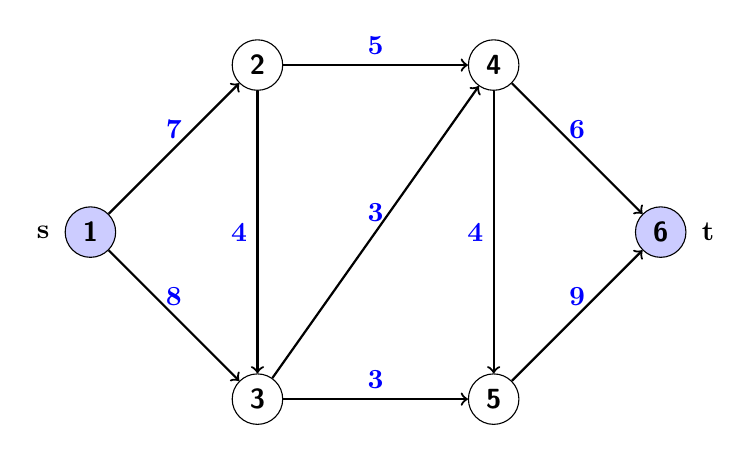
\begin{tikzpicture}
 [main node/.style={node distance=3cm, circle,fill=blue!20,draw,font=\sffamily\bfseries}, 
  normal node/.style={node distance=3cm, circle,fill=white!20,draw,font=\sffamily\bfseries}]
 
\node[main node] (1){1};
\node[normal node] (2)[above right of=1] {2};
\node[normal node] (3) [below right of=1] {3};
\node[normal node] (4) [right of=2] {4};
\node[normal node] (5) [right of=3] {5};
\node[main node] (6) [below right of=4] {6};
\node (s) [node distance=6mm, left of=1]{$\mathbf{s}$};
\node (t) [node distance=6mm, right of=6]{$\mathbf{t}$};
  
\path
  (1) edge [->, thick] node [above] {\textcolor{blue}{$\mathbf{7}$}} (2)
  (1) edge [->, thick] node [above] {\textcolor{blue}{$\mathbf{8}$}} (3)
  (2) edge [->, thick] node [left]      {\textcolor{blue}{$\mathbf{4}$}} (3) 
  (2) edge [->, thick] node [above] {\textcolor{blue}{$\mathbf{5}$}} (4)
  (3) edge [->, thick] node [above] {\textcolor{blue}{$\mathbf{3}$}} (4)
  (3) edge [->, thick] node [above] {\textcolor{blue}{$\mathbf{3}$}} (5) 
  (4) edge [->, thick] node [left]      {\textcolor{blue}{$\mathbf{4}$}} (5)
  (4) edge [->, thick] node [above] {\textcolor{blue}{$\mathbf{6}$}} (6) 
  (5) edge [->, thick] node [above] {\textcolor{blue}{$\mathbf{9}$}} (6);

\end{tikzpicture}
\caption{The flow network $N$}\label{fln-sem-5-1}
\end{center}
\end{figure}


Give two iterations of the Ford-Fulkerson algorithm for $N$, considering 
the path $P=1246$ for the first augmentation and $Q=1356$ for the second augmentation.
\solution{The initial flow is $f:=0$, hence the residual network coincides with $N$.

Let us consider the $s$-$t$ path $P=1246$ as an $f$-augmenting path. Then 
\[\gamma=\min_{e\in A(P)}c_f(e)=\min\{7,5,6\}=5.\] 
Thus, the algorithm augments $f$ along $P$ with 5 units, i.e. we replace $f$ with 
$f_1:=f_P^\gamma$.

\begin{figure}[h!]
\begin{center}
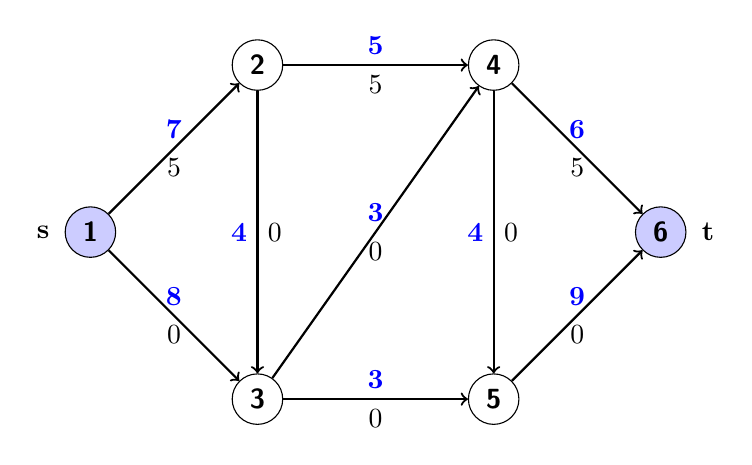
\begin{tikzpicture}
 [main node/.style={node distance=3cm, circle,fill=blue!20,draw,font=\sffamily\bfseries}, 
  normal node/.style={node distance=3cm, circle,fill=white!20,draw,font=\sffamily\bfseries}]
  
\node[main node] (1){1};
   \node[normal node] (2)[above right of=1] {2};
\node[normal node] (3) [below right of=1] {3};
 \node[normal node] (4) [right of=2] {4};
 \node[normal node] (5) [right of=3] {5};
  
  \node[main node] (6) [below right of=4] {6};

  \node (s) [node distance=6mm, left of=1]{$\mathbf{s}$};
  \node (t) [node distance=6mm, right of=6]{$\mathbf{t}$};  
   
\path
  (1) edge [->, thick] node [above] {\textcolor{blue}{$\mathbf{7}$}} node [below] {5} (2)
  (1) edge [->, thick] node [above] {\textcolor{blue}{$\mathbf{8}$}} node [below] {0} (3)
  (2) edge [->, thick] node [left] {\textcolor{blue}{$\mathbf{4}$}} node [right] {0} (3) 
  (2) edge [->, thick] node [above] {\textcolor{blue}{$\mathbf{5}$}} node [below] {5} (4)
  (3) edge [->, thick] node [above] {\textcolor{blue}{$\mathbf{3}$}} node [below] {0} (4)
  (3) edge [->, thick] node [above] {\textcolor{blue}{$\mathbf{3}$}} node [below] {0} (5) 
  (4) edge [->, thick] node [left] {\textcolor{blue}{$\mathbf{4}$}} node [right] {0} (5)
  (4) edge [->, thick] node [above] {\textcolor{blue}{$\mathbf{6}$}} node [below] {5} (6) 
  (5) edge [->, thick] node [above] {\textcolor{blue}{$\mathbf{9}$}} node [below] {0} (6);
  
\end{tikzpicture}
\caption{The flow network $N$ with the flow $f_1$}
\end{center}
\end{figure}

After the first augmentation, we get the following residual graph $D_{f_1}$ and residual capacities $c_{f_1}$:


\begin{figure}[h!]

\begin{center}
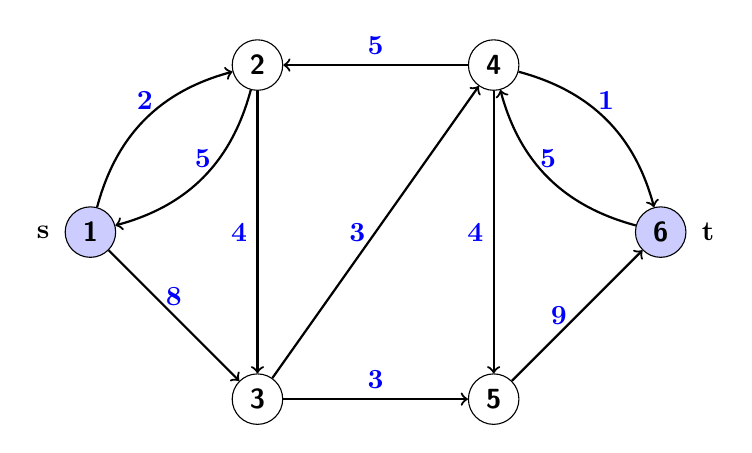
\begin{tikzpicture}
 [main node/.style={node distance=3cm, circle,fill=blue!20,draw,font=\sffamily\bfseries}, 
  normal node/.style={node distance=3cm, circle,fill=white!20,draw,font=\sffamily\bfseries}]
  
\node[main node] (1){1};
   \node[normal node] (2)[above right of=1] {2};
\node[normal node] (3) [below right of=1] {3};
 \node[normal node] (4) [right of=2] {4};
 \node[normal node] (5) [right of=3] {5};
  
  \node[main node] (6) [below right of=4] {6};

  \node (s) [node distance=6mm, left of=1]{$\mathbf{s}$};
  \node (t) [node distance=6mm, right of=6]{$\mathbf{t}$};  
   
\path
  (1) edge [->, thick, bend left] node [above] {\textcolor{blue}{$\mathbf{2}$}}  (2)
  (2) edge [->, thick, bend left] node [above] {\textcolor{blue}{$\mathbf{5}$}}  (1)
  
  (4) edge [->, thick, bend left] node [above] {\textcolor{blue}{$\mathbf{1}$}}  (6) 
  (6) edge [->, thick, bend left] node [above] {\textcolor{blue}{$\mathbf{5}$}}  (4) 
  
  (4) edge [->, thick] node [above] {\textcolor{blue}{$\mathbf{5}$}} (2)
  
  (1) edge [->, thick] node [above] {\textcolor{blue}{$\mathbf{8}$}} (3)
  (2) edge [->, thick] node [left] {\textcolor{blue}{$\mathbf{4}$}} (3)
  (4) edge [->, thick] node [left] {\textcolor{blue}{$\mathbf{4}$}}  (5)
  (3) edge [->, thick] node [left] {\textcolor{blue}{$\mathbf{3}$}}  (4) 
  (3) edge [->, thick] node [above] {\textcolor{blue}{$\mathbf{3}$}}  (5) 
  (5) edge [->, thick] node [left] {\textcolor{blue}{$\mathbf{9}$}}  (6);
  
       
\end{tikzpicture}
\caption{The residual graph $D_{f_1}$}
\end{center}
\end{figure}

Let us consider at the second iteration the $s$-$t$ path $Q=1356$ as an $f_1$-augmenting path. Then 
\[\gamma=\min_{e\in A(P)}c_{f_1}(e)=\min\{8,3,9\}=3.\] 
Thus, the algorithm augments $f$ along $Q$ with $3$ units, i.e. we replace $f_1$ with 
$f_2:={f_1}_Q^\gamma$.
\begin{figure}[h!]
\begin{center}
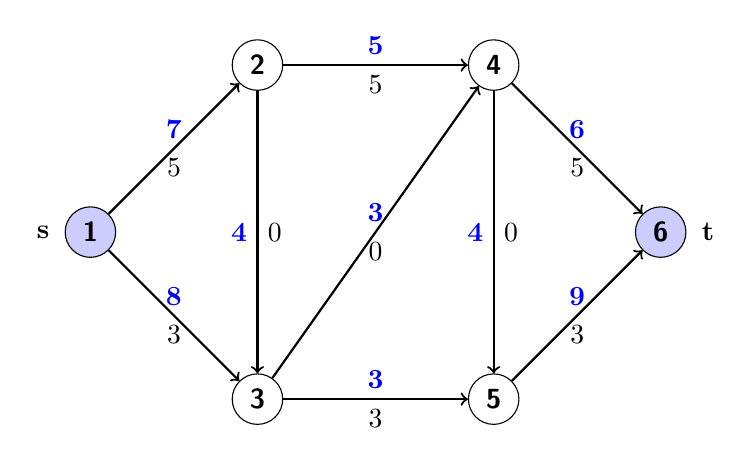
\begin{tikzpicture}
 [main node/.style={node distance=3cm, circle,fill=blue!20,draw,font=\sffamily\bfseries}, 
  normal node/.style={node distance=3cm, circle,fill=white!20,draw,font=\sffamily\bfseries}]
  
\node[main node] (1){1};
   \node[normal node] (2)[above right of=1] {2};
\node[normal node] (3) [below right of=1] {3};
 \node[normal node] (4) [right of=2] {4};
 \node[normal node] (5) [right of=3] {5};
  
  \node[main node] (6) [below right of=4] {6};

  \node (s) [node distance=6mm, left of=1]{$\mathbf{s}$};
  \node (t) [node distance=6mm, right of=6]{$\mathbf{t}$};  
   
\path
  (1) edge [->, thick] node [above] {\textcolor{blue}{$\mathbf{7}$}} node [below] {5} (2)
  (1) edge [->, thick] node [above] {\textcolor{blue}{$\mathbf{8}$}} node [below] {3} (3)
  (2) edge [->, thick] node [left] {\textcolor{blue}{$\mathbf{4}$}} node [right] {0} (3) 
  (2) edge [->, thick] node [above] {\textcolor{blue}{$\mathbf{5}$}} node [below] {5} (4)
  (3) edge [->, thick] node [above] {\textcolor{blue}{$\mathbf{3}$}} node [below] {0} (4)
  (3) edge [->, thick] node [above] {\textcolor{blue}{$\mathbf{3}$}} node [below] {3} (5) 
  (4) edge [->, thick] node [left] {\textcolor{blue}{$\mathbf{4}$}} node [right] {0} (5)
  (4) edge [->, thick] node [above] {\textcolor{blue}{$\mathbf{6}$}} node [below] {5} (6) 
  (5) edge [->, thick] node [above] {\textcolor{blue}{$\mathbf{9}$}} node [below] {3} (6);
  
\end{tikzpicture}
\caption{The flow network $N$ with the flow $f_2$}
\end{center}
\end{figure}

After the second augmentation, we get the following residual graph $D_{f_2}$ and residual capacities $c_{f_2}$:


\begin{figure}[h!]

\begin{center}
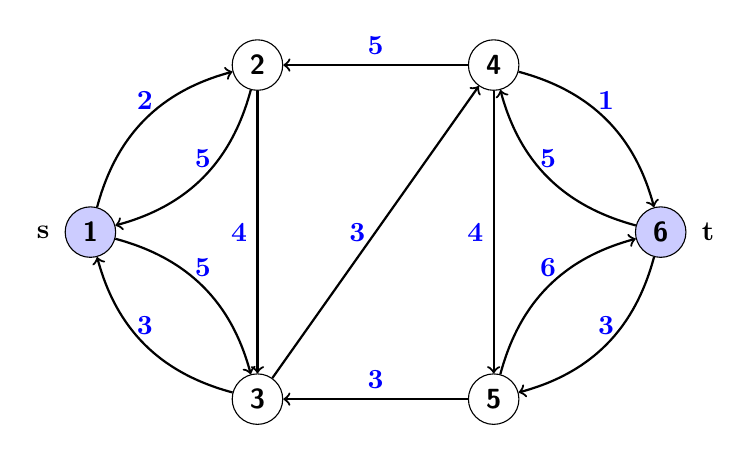
\begin{tikzpicture}
 [main node/.style={node distance=3cm, circle,fill=blue!20,draw,font=\sffamily\bfseries}, 
  normal node/.style={node distance=3cm, circle,fill=white!20,draw,font=\sffamily\bfseries}]
  
\node[main node] (1){1};
   \node[normal node] (2)[above right of=1] {2};
\node[normal node] (3) [below right of=1] {3};
 \node[normal node] (4) [right of=2] {4};
 \node[normal node] (5) [right of=3] {5};
  
  \node[main node] (6) [below right of=4] {6};

  \node (s) [node distance=6mm, left of=1]{$\mathbf{s}$};
  \node (t) [node distance=6mm, right of=6]{$\mathbf{t}$};  
   
\path
  (1) edge [->, thick, bend left] node [above] {\textcolor{blue}{$\mathbf{2}$}}  (2)
  (2) edge [->, thick, bend left] node [above] {\textcolor{blue}{$\mathbf{5}$}}  (1)
  
  (4) edge [->, thick, bend left] node [above] {\textcolor{blue}{$\mathbf{1}$}}  (6) 
  (6) edge [->, thick, bend left] node [above] {\textcolor{blue}{$\mathbf{5}$}}  (4) 
  
  (4) edge [->, thick] node [above] {\textcolor{blue}{$\mathbf{5}$}} (2)
  
  (1) edge [->, thick, bend left] node [above] {\textcolor{blue}{$\mathbf{5}$}}  (3)
  (3) edge [->, thick, bend left] node [above] {\textcolor{blue}{$\mathbf{3}$}}  (1)
  
  (5) edge [->, thick] node [above] {\textcolor{blue}{$\mathbf{3}$}}  (3) 
   (4) edge [->, thick] node [left] {\textcolor{blue}{$\mathbf{4}$}}  (5)
  
  (5) edge [->, thick, bend left] node [above] {\textcolor{blue}{$\mathbf{6}$}}  (6)
  (6) edge [->, thick, bend left] node [above] {\textcolor{blue}{$\mathbf{3}$}}  (5)
  

  (2) edge [->, thick] node [left] {\textcolor{blue}{$\mathbf{4}$}} (3)
  (3) edge [->, thick] node [left] {\textcolor{blue}{$\mathbf{3}$}}  (4);
  
       
\end{tikzpicture}
\caption{The residual graph $D_{f_2}$}
\end{center}
\end{figure}
}

%\newpage 


\semex
Figure \ref{fln-f-sem-5} represents a flow network $N$ and an $s$-$t$ flow $f$ for  $N$. 

\begin{figure}[h!]
\begin{center}
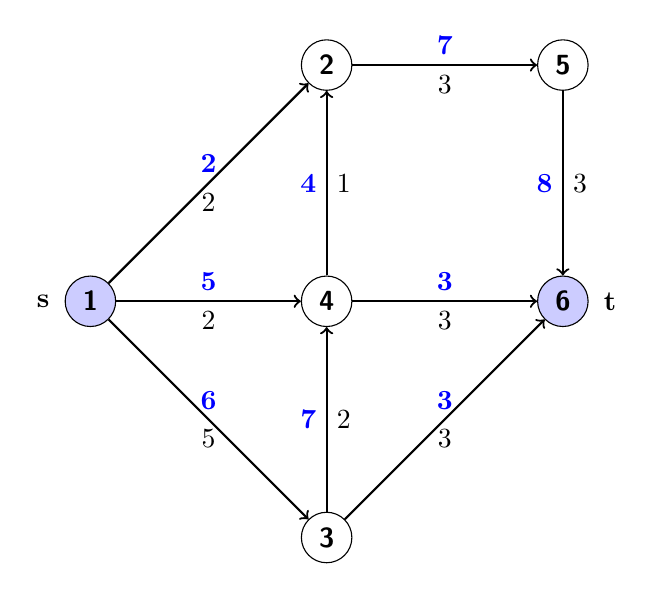
\begin{tikzpicture}
 [main node/.style={node distance=3cm, circle,fill=blue!20,draw,font=\sffamily\bfseries}, 
  normal node/.style={node distance=3cm, circle,fill=white!20,draw,font=\sffamily\bfseries}]
 
 \node[normal node] (2){2};
 \node[normal node] (4) [below of=2] {4};
\node[main  node] (1)[ left of=4] {1};
\node[normal node] (3) [below of=4] {3};
\node[main node] (6) [right of=4] {6};

\node[normal node] (5) [right of=2] {5};

\node (s) [node distance=6mm, left of=1]{$\mathbf{s}$};
\node (t) [node distance=6mm, right of=6]{$\mathbf{t}$};

\path
  (1) edge [->, thick] node [above] {\textcolor{blue}{$\mathbf{2}$}} node [below] {2} (2)
  (1) edge [->, thick] node [above] {\textcolor{blue}{$\mathbf{6}$}} node [below] {5} (3)
   (1) edge [->, thick] node [above] {\textcolor{blue}{$\mathbf{5}$}} node [below] {2} (4)
   
 
  (2) edge [->, thick] node [above] {\textcolor{blue}{$\mathbf{7}$}} node [below] {3} (5)
  
  (3) edge [->, thick] node [left] {\textcolor{blue}{$\mathbf{7}$}} node [right] {2} (4)
  (3) edge [->, thick] node [above] {\textcolor{blue}{$\mathbf{3}$}} node [below] {3} (6)
  
   
    (4) edge [->, thick] node [left] {\textcolor{blue}{$\mathbf{4}$}} node [right] {1} (2)
    (4) edge [->, thick] node [above] {\textcolor{blue}{$\mathbf{3}$}} node [below] {3} (6)
   
     (5) edge [->, thick] node [left] {\textcolor{blue}{$\mathbf{8}$}} node [right] {3} (6);
  
    
\end{tikzpicture}
\caption{The flow network $N$ with the flow $f$}\label{fln-f-sem-5}
\end{center}
\end{figure}
\be
\item Represent the residual graph  $D_f$ and the residual capacities $c_f$.
\item Choose an $f$-augmenting path $P$ of minimum length and compute the flow 
$g:=f_P^\gamma$, where $\gamma=\min_{e\in A(P)}c_f(e)$. 
\item Represent the residual graph  $D_g$ and the residual capacities  $c_g$. 
Can you find an   $s$-$t$ path in $D_g$?
\item What is the maximum value of and $s$-$t$ flow for $N$? 
\item Give an example of an $s$-$t$ cut in  $N$ of minimum capacity.
\ee
\solution{
\be
\item The residual graph $D_f$ and residual capacities $c_f$ are given in Figure \ref{fln-f-sem-5-df}.

\begin{figure}[h!]
\begin{center}
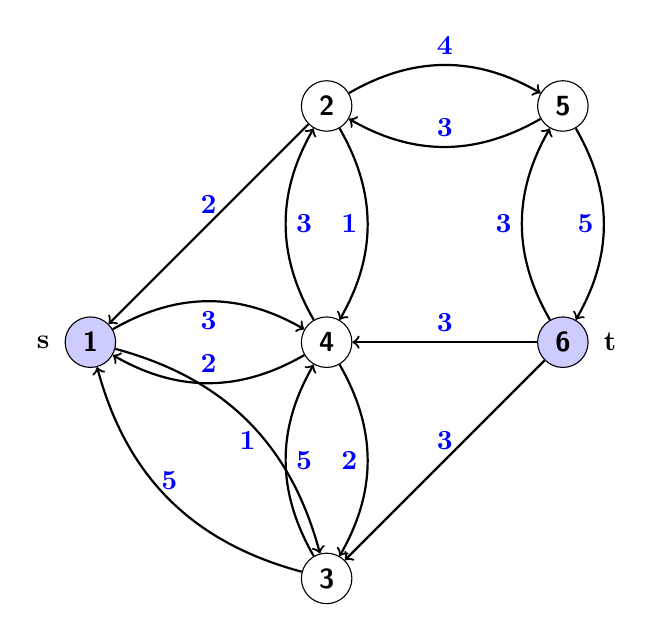
\begin{tikzpicture}
 [main node/.style={node distance=3cm, circle,fill=blue!20,draw,font=\sffamily\bfseries}, 
  normal node/.style={node distance=3cm, circle,fill=white!20,draw,font=\sffamily\bfseries}]
 
\node[normal node] (2){2};
 \node[normal node] (4) [below of=2] {4};
\node[main  node] (1)[ left of=4] {1};
\node[normal node] (3) [below of=4] {3};
\node[main node] (6) [right of=4] {6};

\node[normal node] (5) [right of=2] {5};

\node (s) [node distance=6mm, left of=1]{$\mathbf{s}$};
\node (t) [node distance=6mm, right of=6]{$\mathbf{t}$};

\path
  (1) edge  [->, thick, bend left]  node [below] {\textcolor{blue}{$\mathbf{1}$}}  (3)
   (3) edge  [->, thick, bend left]  node [above] {\textcolor{blue}{$\mathbf{5}$}}  (1)
   
   (1) edge [->, thick, bend left] node [below] {\textcolor{blue}{$\mathbf{3}$}}  (4)
     (4) edge [->, thick, bend left] node [above] {\textcolor{blue}{$\mathbf{2}$}}  (1)
   
  (2) edge [->, thick] node [above] {\textcolor{blue}{$\mathbf{2}$}}  (1)
  
   (6) edge [->, thick] node [above] {\textcolor{blue}{$\mathbf{3}$}}  (3)
  
     (3) edge  [->, thick, bend left]  node [right] {\textcolor{blue}{$\mathbf{5}$}}  (4)
   (4) edge  [->, thick, bend left]  node [left] {\textcolor{blue}{$\mathbf{2}$}}  (3)

  (4) edge  [->, thick, bend left]  node [right] {\textcolor{blue}{$\mathbf{3}$}}  (2)
   (2) edge  [->, thick, bend left]  node [left] {\textcolor{blue}{$\mathbf{1}$}}  (4)
   
   (2) edge  [->, thick, bend left]  node [above] {\textcolor{blue}{$\mathbf{4}$}}  (5)
   (5) edge  [->, thick, bend left]  node [above] {\textcolor{blue}{$\mathbf{3}$}}  (2)


  (5) edge  [->, thick, bend left]  node [left] {\textcolor{blue}{$\mathbf{5}$}}  (6)
   (6) edge  [->, thick, bend left]  node [left] {\textcolor{blue}{$\mathbf{3}$}}  (5)


  
            
       (6) edge [->, thick] node [above] {\textcolor{blue}{$\mathbf{3}$}}  (4);
  
    
\end{tikzpicture}
\caption{The residual graph $D_f$}\label{fln-f-sem-5-df}
\end{center}
\end{figure}

\item  The $s$-$t$ path of minimum length is $P=14256$, so we choose it as an 
$f$-augmenting path. Then  
\[\gamma=\min_{e\in A(P)}c_f(e)=\min\{3,4,5\}=3.\] 
The flow network $N$ with the flow $g:=f_P^\gamma$ is given in Figure \ref{fln-f-sem-5-g}.


\begin{figure}[h!]
\begin{center}
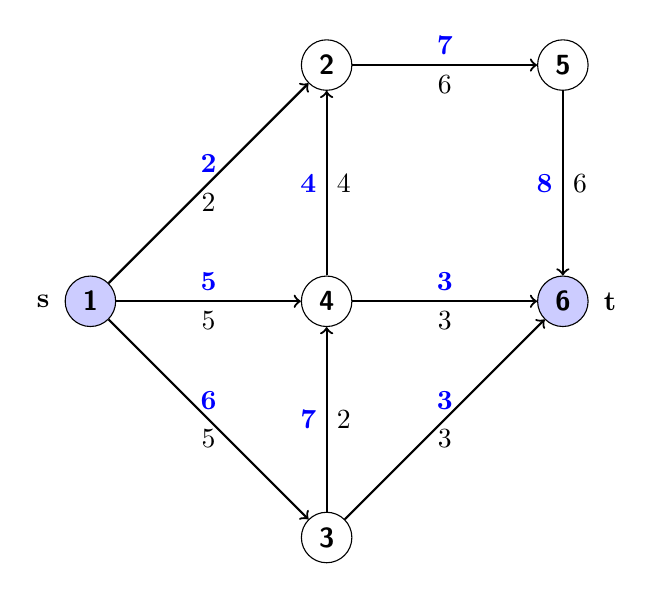
\begin{tikzpicture}
 [main node/.style={node distance=3cm, circle,fill=blue!20,draw,font=\sffamily\bfseries}, 
  normal node/.style={node distance=3cm, circle,fill=white!20,draw,font=\sffamily\bfseries}]
 
 \node[normal node] (2){2};
 \node[normal node] (4) [below of=2] {4};
\node[main  node] (1)[ left of=4] {1};
\node[normal node] (3) [below of=4] {3};
\node[main node] (6) [right of=4] {6};

\node[normal node] (5) [right of=2] {5};

\node (s) [node distance=6mm, left of=1]{$\mathbf{s}$};
\node (t) [node distance=6mm, right of=6]{$\mathbf{t}$};


\path
  (1) edge [->, thick] node [above] {\textcolor{blue}{$\mathbf{2}$}} node [below] {2} (2)
  (1) edge [->, thick] node [above] {\textcolor{blue}{$\mathbf{6}$}} node [below] {5} (3)
   (1) edge [->, thick] node [above] {\textcolor{blue}{$\mathbf{5}$}} node [below] {5} (4)
   
 
  (2) edge [->, thick] node [above] {\textcolor{blue}{$\mathbf{7}$}} node [below] {6} (5)
  
  (3) edge [->, thick] node [left] {\textcolor{blue}{$\mathbf{7}$}} node [right] {2} (4)
  (3) edge [->, thick] node [above] {\textcolor{blue}{$\mathbf{3}$}} node [below] {3} (6)
  
   
    (4) edge [->, thick] node [left] {\textcolor{blue}{$\mathbf{4}$}} node [right] {4} (2)
    (4) edge [->, thick] node [above] {\textcolor{blue}{$\mathbf{3}$}} node [below] {3} (6)
   
     (5) edge [->, thick] node [left] {\textcolor{blue}{$\mathbf{8}$}} node [right] {6} (6);
  
    
\end{tikzpicture}
\caption{The flow network $N$ with the flow $g$}\label{fln-f-sem-5-g}
\end{center}
\end{figure}

\item The residual graph $D_g$ and residual capacities $c_g$ are given in Figure \ref{fln-f-sem-5-dg}.

\begin{figure}[h!]
\begin{center}
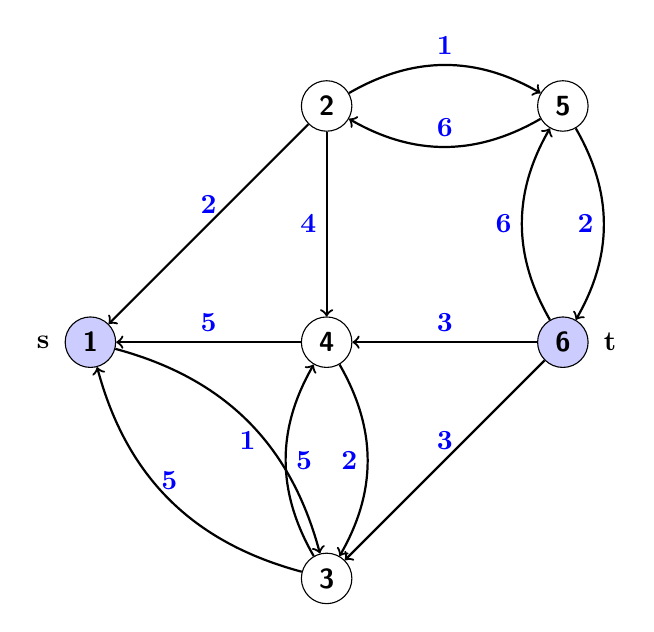
\begin{tikzpicture}
 [main node/.style={node distance=3cm, circle,fill=blue!20,draw,font=\sffamily\bfseries}, 
  normal node/.style={node distance=3cm, circle,fill=white!20,draw,font=\sffamily\bfseries}]
 
 \node[normal node] (2){2};
 \node[normal node] (4) [below of=2] {4};
\node[main  node] (1)[ left of=4] {1};
\node[normal node] (3) [below of=4] {3};
\node[main node] (6) [right of=4] {6};

\node[normal node] (5) [right of=2] {5};

\node (s) [node distance=6mm, left of=1]{$\mathbf{s}$};
\node (t) [node distance=6mm, right of=6]{$\mathbf{t}$};

\path
  (1) edge  [->, thick, bend left]  node [below] {\textcolor{blue}{$\mathbf{1}$}}  (3)
   (3) edge  [->, thick, bend left]  node [above] {\textcolor{blue}{$\mathbf{5}$}}  (1)
   
      (4) edge [->, thick] node [above] {\textcolor{blue}{$\mathbf{5}$}}  (1)
   
  (2) edge [->, thick] node [above] {\textcolor{blue}{$\mathbf{2}$}}  (1)
  
   (6) edge [->, thick] node [above] {\textcolor{blue}{$\mathbf{3}$}}  (3)
  
     (3) edge  [->, thick, bend left]  node [right] {\textcolor{blue}{$\mathbf{5}$}}  (4)
   (4) edge  [->, thick, bend left]  node [left] {\textcolor{blue}{$\mathbf{2}$}}  (3)

     (2) edge  [->, thick]  node [left] {\textcolor{blue}{$\mathbf{4}$}}  (4)
   
   (2) edge  [->, thick, bend left]  node [above] {\textcolor{blue}{$\mathbf{1}$}}  (5)
   (5) edge  [->, thick, bend left]  node [above] {\textcolor{blue}{$\mathbf{6}$}}  (2)


  (5) edge  [->, thick, bend left]  node [left] {\textcolor{blue}{$\mathbf{2}$}}  (6)
   (6) edge  [->, thick, bend left]  node [left] {\textcolor{blue}{$\mathbf{6}$}}  (5)


  
            
       (6) edge [->, thick] node [above] {\textcolor{blue}{$\mathbf{3}$}}  (4);
    
\end{tikzpicture}
\caption{The residual graph $D_g$}\label{fln-f-sem-5-dg}
\end{center}
\end{figure}

It is obvious that there are no $s$-$t$ paths in $D_g$. 
\item By Theorem 3.2.4, 
it follows that $g$ is a maximum flow. Hence, the maximal value of an $s$-$t$ flow is 
$\text{value}(g)=5+2+5=12$.
\item By the Max-Flow Min-Cut Theorem 3.0.11,  the minimum capacity of an $s$-$t$ cut is $12$. Apply 
Proposition 3.2.3. to get that 
an $s$-$t$ cut having this capacity is $$\{(1,2), (4,2), (4,6),(3,6)\}=\delta^{out}(U),$$ where $U=\{1,3,4\}$ is the set of vertices reachable in $D_g$ from $1$.
\ee
}

\semex
Prove Proposition 3.4.2..
\solution{Apply the Flow Decomposition Theorem 3.4.1. Then there exist $K,L\in\Z_+$, positive numbers 
$w_1,\ldots, w_K, \mu_1,\ldots,\mu_L$, $s$-$t$
paths $P_1,\ldots, P_K$ and circuits $C_1,\ldots, C_L$ such that  
\[f=\sum_{i=1}^K w_i\chi^{P_i}+\sum_{j=1}^L \mu_j\chi^{C_j}\quad \text{and}\quad \text{value}(f)=\sum_{i=1}^K w_i. \]
Furthermore, the $w_i$'s, $\mu_j$'s are positive integers. Since $f$ is a $\{0,1\}$-flow,
we must have $w_i=\mu_j=1$ for all $i,j$. Thus,
\[f=\sum_{i=1}^K \chi^{P_i}+\sum_{j=1}^L \chi^{C_j}\quad \text{and}\quad \text{value}(f)=K. \]

It remains to show that the family 
$\cF=\{P_1,\ldots, P_K,C_1,\ldots, C_L\}$ is arc-disjoint. If $Q_1,Q_2\in \cF$ have an arc $a$ 
in common, then $f(a)\geq \chi^{Q_1}(a)+\chi^{Q_2}(a)=2$, which contradicts the fact that 
$f$ is a $\{0,1\}$-flow.
}


\semex
For any $s$-$t$ path $P$ in $D$, prove that $\chi^P$ satisfies the flow conservation law at every $v\ne s,t$
and that $\text{value}(\chi^P)=1$.
\solution{
If $P=st$, then $\chi^P(a)=0$ for all $a\ne (s,t)$, hence $in_{\chi^P}(v)=out_{\chi^P}(v)=0$ for all
$v\ne s,t$. Assume that $P=sv_1\ldots v_kt$ with $k\geq 1$. Let us denote $v_0:=s, v_{k+1}:=t$. 
Then $\chi^P((s,v_1))=\chi^P((v_1,v_2))=
\ldots =\chi^P((v_{k-1},v_k))=\chi^P((v_k,t))=1$ and $\chi^P(a)=0$ for all the other arcs $a$.
For an arbitrary $v\ne s,t$ we have two cases:
\be
\item $v\notin P$. Then $in_{\chi^P}(v)=out_{\chi^P}(v)=0$.
\item $v=v_i, i=1,\ldots, k$. Then 
\bua
in_{\chi^P}(v_i)=\sum_{a\in\delta^{in}(v_i)}\chi^P(a)=\chi^P((v_{i-1},v_i))+0=1, \\
out_{\chi^P}(v_i)=\sum_{a\in\delta^{out}(v_i)}\chi^P(a)=\chi^P((v_i,v_{i+1}))+0=1.
\eua
\ee
Finally, 
\bua
\text{value}(\chi^P)=out_{\chi^P}(s)-in_{\chi^P}(s)=\chi^P((s,v_1))-0=1.
\eua
}

\end{document}




\end{document}